\documentclass[titlepage]{article}
\usepackage[tmargin=1in,bmargin=1in,lmargin=1.25in,rmargin=1.25in]{geometry}
\usepackage[utf8]{inputenc}
\usepackage[english]{babel}
\usepackage{eurosym}


%\usepackage{keyval}
\usepackage{graphicx}
\usepackage{usebib}
\usepackage{bibentry}
\usepackage{caption}
\usepackage{array}
\usepackage{nameref}
\newcolumntype{P}[1]{>{\raggedright\arraybackslash}p{#1}}
\usepackage{xcolor}
\usepackage{pdfpages}
\usepackage{enumitem}
\usepackage{makecell}

\newcommand\todo[1]{\textcolor{red}{#1}}
\newenvironment{itemize*}%
  {\begin{itemize}%
    \setlength{\itemsep}{0pt}%
    \setlength{\parskip}{0pt}}%
  {\end{itemize}}


\usepackage[numbers,sort]{natbib}
\usepackage{xcolor}
\usepackage{ragged2e}
\usepackage{multirow}
\bibliographystyle{abbrvnat}

\definecolor{myred}{RGB}{146, 33, 33}
\newcommand{\heading}[1] {
\vspace*{0.7cm}\noindent \textcolor{myred}{\large{\textbf{\uppercase{{#1}}}}} \\[-5pt]
\noindent\makebox[\linewidth]{\rule{\textwidth}{0.4pt}\vspace*{0.2cm}}
}

\newcommand{\subheading}[1] {\vspace*{0.5cm}\noindent \uppercase{\textbf{#1}}}
\usepackage[hidelinks]{hyperref}

\hypersetup{
    colorlinks = true,
   allcolors = myred}
   
\usepackage[T1]{fontenc}
\usepackage[utf8]{inputenc} 
 \usepackage{helvet}
  \fontfamily{lmodern}
  \renewcommand{\familydefault}{\sfdefault}

\begin{document}
\nobibliography{ref}


\centerline{\huge{\textcolor{myred}{\textbf{Curriculum Vitae}}}}
\vspace{0.5cm}
\centerline{\Large{\textbf{Prof. Dr. Henrik Leopold}}}
\vspace{1.5cm}

\begin{tabular}{P{3cm}P{5.0cm}l}
Name:					&  Henrik Leopold  & \multirow{9}{*}{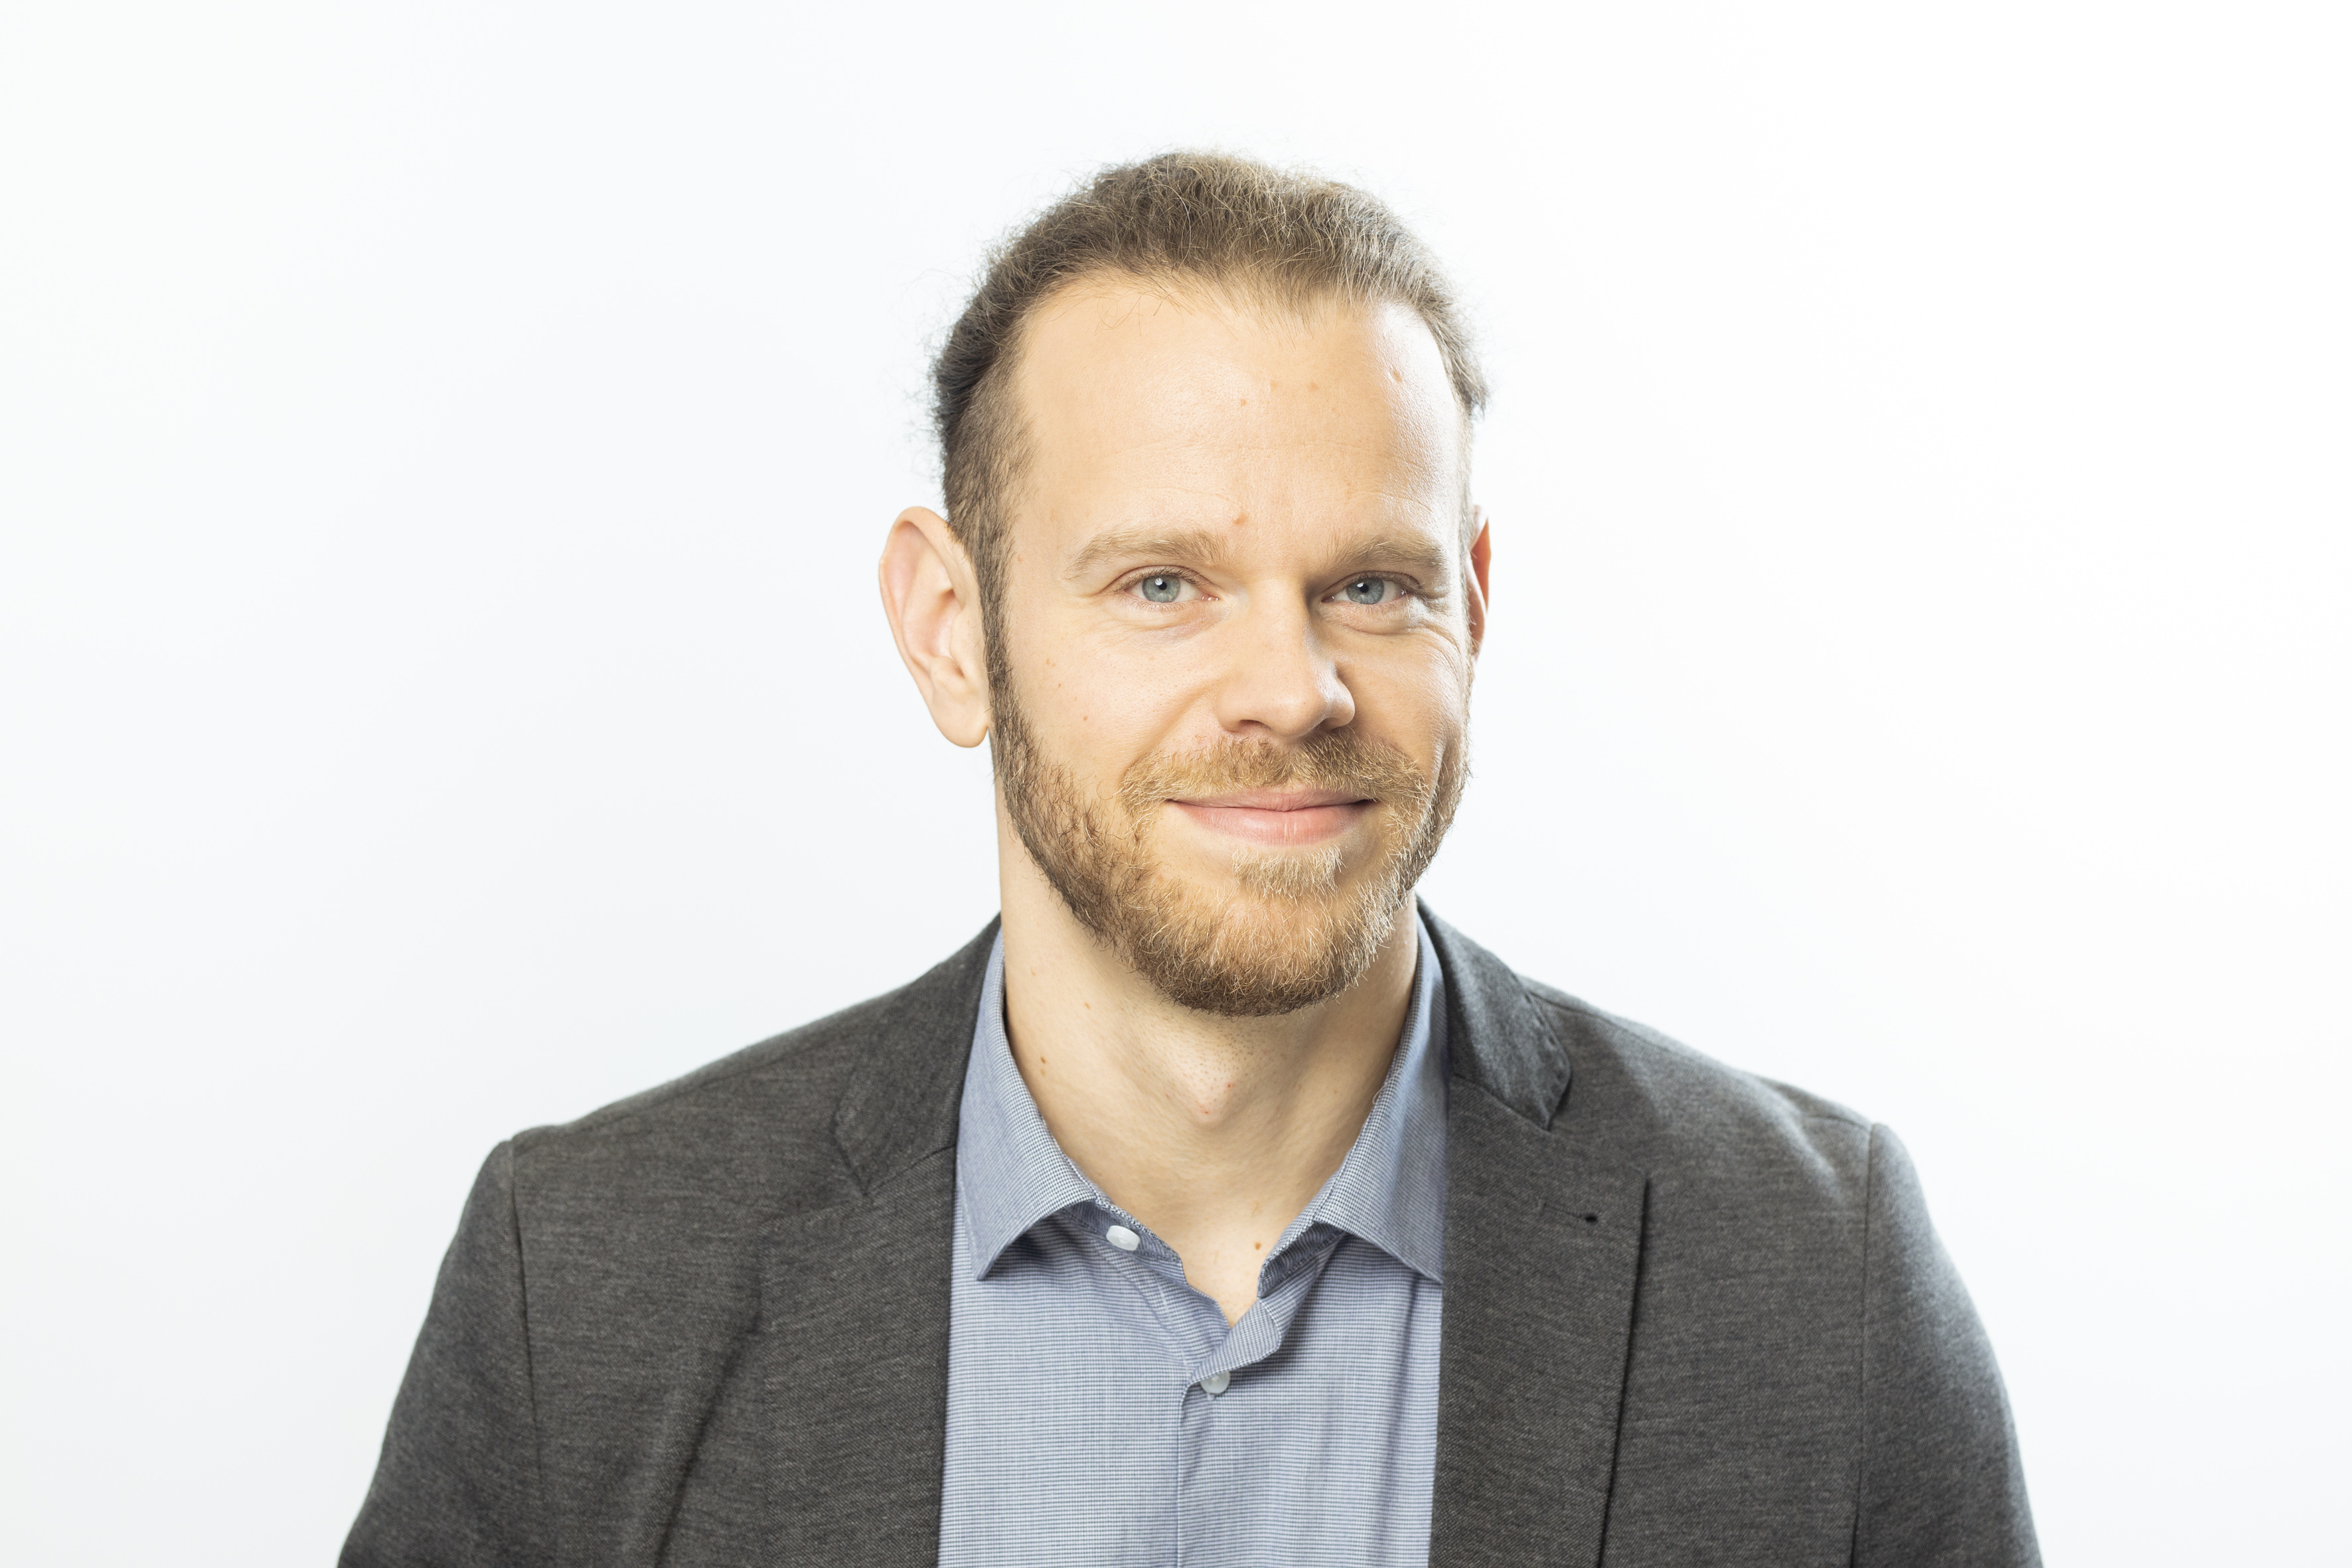
\includegraphics[scale=0.18]{figures/HLeopold.jpg}} \\
Date of Birth: 		& 24/05/1986 \\
Place of Birth: 		& Leipzig, Germany \\
Marital Status: 		& Married to Franziska Leopold \\
Children:				& Jona Milian, 2 years \\
Address:				& Holteistraße 14, 10245 Berlin \\
Mobile: 				& +49 (0)175 5631 251 \\
E-Mail: 				& \href{mailto:henrik.leopold@the-klu.org}{henrik.leopold@the-klu.org} \\
Web:						& \href{www.henrikleopold.com}{www.henrikleopold.com} \\
\end{tabular}

\heading{Education}

\raggedright
\begin{tabular}{P{3cm}P{12cm}}
\
01/2011   													& \textbf{Ph.D. in Information Systems} \\
\hspace*{0.4cm}$\Rightarrow$  07/2013	& Thesis title: ``Natural Language in Business Process Models'' \\
																	& Humboldt University of Berlin \\
																	& Advisor: Prof. Dr. Jan Mendling (WU Vienna) \\
																	& Degree: Dr. rer. pol. (summa cum laude) \\
																	\\
10/2008														& \textbf{Study of Information Systems} \\
\hspace*{0.4cm}$\Rightarrow$  10/2010	&  Humboldt University of Berlin  \\																	
																	&  Title of Master Thesis: ``Modularization of Process Models Using Natural Language Techniques'' \\
																	& Degree: Master of Science \\
																	\\
10/2005 														& \textbf{Study of Information Systems} \\
\hspace*{0.4cm}$\Rightarrow$  09/2008	&	Berlin School of Economics and Law (Dual study program) \\															
																	& Degree: Bachelor of Science \\
																	\\
08/1998														& \textbf{High School} \\ 
\hspace*{0.4cm}$\Rightarrow$  07/2005	& Max-Reinhardt-Gymnasium, Berlin \\																
																	& Degree: Abitur (High School Diploma) \\
\end{tabular}


\heading{Appointments}


\raggedright
\begin{tabular}{P{3cm}P{12cm}}
06/2020														& \textbf{Associate Professor (with tenure)} \\
\hspace*{0.4cm}$\Rightarrow$ today			&  Kühne Logistics University \\
																	& Area:  Data Science and Business Intelligence\\
																	\\																
02/2019														& \textbf{Senior Researcher} \\
\hspace*{0.4cm}$\Rightarrow$ today			& Hasso Plattner Institute, University Potsdam   \\
																	& Associated group: Business Process Technology (Prof. Dr. Mathias Weske) \\
																	\\																	
02/2019														& \textbf{Assistant Professor} \\
\hspace*{0.4cm}$\Rightarrow$ 06/2020	&  Kühne Logistics University \\
																	& Area:  Data Science and Business Intelligence\\
\end{tabular}
\raggedright
\begin{tabular}{P{3cm}P{12cm}}																	
02/2015   													& \textbf{Assistant Professor} \\
\hspace*{0.4cm}$\Rightarrow$  01/2019	& VU Amsterdam, Amsterdam, The Netherlands \\
																	& Department of Computer Science\\
																	\\
04/2014   													& \textbf{Assistant Professor} \\
\hspace*{0.4cm}$\Rightarrow$  01/2015	& WU Vienna, Vienna, Austria \\
																	& Institute for Information Business \\
																	\\
01/2011   													& \textbf{Research Assistant} \\
\hspace*{0.4cm}$\Rightarrow$  01/2015	& Humboldt University of Berlin, Berlin, Germany \\
																	& Institute of Information Systems \\
																	\\
10/2005   													& \textbf{Student Employee} \\
\hspace*{0.4cm}$\Rightarrow$  12/2010	& Bayer Healthcare AG, Berlin, Germany  \\
																	\\																	
\end{tabular}


%#######################
%			PUBLICATIONS
%#######################
\heading{Ten Most Important Publications}
%\mypartheader{Publications}
\section{Publications}
\noindent My work has been published in several prestigious journals and international conferences, including: 
\begin{itemize}
	\itemsep-0.2em
	
	\item Information Systems  (IS) -- 6x
	
	\item Decision support systems (DSS) -- 2x
	
	\item IEEE Transactions on Knowledge and Data Engineering (TKDE) -- 1x
	
	\item Data and Knowledge Engineering  (DKE) -- 2x
	
	\item Int.\ Conf.\ on Advanced Information Systems Engineering (CAISE)	 -- 7x
	
	\item Int.\ Conf.\ on Business Process Management (BPM) --  5x

	\item Int.\ Conf.\ on Computational Linguistics (COLING) -- 1x
	
	\item ACM Int.\ Conf.\ on Management of Data (SIGMOD) -- 1x 
	
	
\end{itemize}
\smallskip
Pre-print versions of all my publications are available at \href{https://www.hanvanderaa.com/publications}{www.hanvanderaa.com/publications}\\

%\section{Bibliographic Profile}
%\begin{figure}[!h]
%	\centering
%	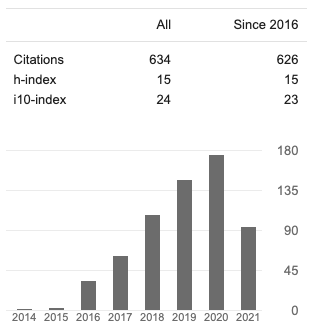
\includegraphics[width=0.38\linewidth]{figures/scholarprofile.png}
%\end{figure}
%
%Updated:  June 29, 2021 (source: \href{https://scholar.google.com/citations?user=oFagE6cAAAAJ}{scholar.google.com/citations?user=oFagE6cAAAAJ})\\

\section{Selected Publications}

\begin{enumerate}[label=\arabic*.]
	\itemsep-0.3em
	\mybib{\textbf{Han van der Aa}, Adrian Rebmann, Henrik Leopold}
	{Natural language-based detection of semantic execution anomalies in event logs}
	{Information System 102: 101824, 2021}
	
			\mybib{ Bo Zhao, \textbf{Han van der Aa}, Nguyen Thanh Tam, Nguyen Quoc Viet Hung, Matthias Weidlich} {EIRES Efficient Integration of Remote Data in Event Stream Processing}
	{ACM SIGMOD International Conference on Management of Data (SIGMOD 2021)}
	
	\mybib{ Adrian Rebmann, \textbf{Han van der Aa}} {Extracting Semantic Process Information from the Natural Language in Event Logs} 
	{International Conference on Advanced Information Systems Engineering (CAiSE 2021)}
	
	\mybib{Martin Bauer, \textbf{Han van der Aa}, Matthias Weidlich}
	{Sampling and Approximation Techniques for Efficient Process Conformance Checking}
	{Information Systems 2020 (accepted for publication)}
	
	\mybib{\textbf{Han van der Aa}, Henrik Leopold, Matthias Weidlich}
	{Partial Order Resolution of Event Logs for Process Conformance Checking}
	{Decision Support Systems 136: 113347, 2020}



	\mybib{\textbf{Han van der Aa}, Henrik Leopold, Hajo A. Reijers}{Efficient Process Conformance Checking on the Basis of Uncertain Event-to-Activity Mappings}
{IEEE Transactions on Knowledge and Data Engineering  32(5): 927-940, 2020}

	\mybib{ Stephan A Fahrenkrog-Petersen, \textbf{Han van der Aa}, Matthias Weidlich} {	PRIPEL: Privacy-Preserving Event Log Publishing Including Contextual Information}
{International Conference on Business Process Management (BPM 2020)}

	\mybib{ \textbf{Han van der Aa}, Claudio Di Ciccio, Henrik Leopold and Hajo A Reijers} {Extracting Declarative Process Models from Natural Language} 
{International Conference on Advanced Information Systems Engineering (CAiSE 2019)}
	
\mybib{\textbf{Han van der Aa}, Henrik Leopold, Hajo A. Reijers}{Comparing Textual Descriptions to Process Models – The Automatic Detection of Inconsistencies}
{Information Systems 64: 447-460, 2017}

\mybib{ Claudio Di Ciccio, \textbf{Han van der Aa}, Cristina Cabanillas, Jan Mendling, Johannes Prescher}{Detecting Flight Trajectory Anomalies and Predicting Diversions in Freight Transportation}
{Decision Support Systems 88(1): 1-17, 2016}

\end{enumerate}
%\section{Journal Articles}


%\begin{enumerate}[label=J\arabic*.]
%	\itemsep-0.3em
%	\mybib{\textbf{Han van der Aa}, Adrian Rebmann, Henrik Leopold}
%	{Natural language-based detection of semantic execution anomalies in event logs}
%	{Information System 102: 101824, 2021}
%	
%	
%	\mybib{Martin Bauer, \textbf{Han van der Aa}, Matthias Weidlich}
%	{Sampling and Approximation Techniques for Efficient Process Conformance Checking}
%	{Information Systems 2020 (accepted for publication)}
%	
%	\mybib{\textbf{Han van der Aa}, Henrik Leopold, Matthias Weidlich}
%	{Partial Order Resolution of Event Logs for Process Conformance Checking}
%	{Decision Support Systems 136: 113347, 2020}
%
%		\mybib{Nimrod Busany, \textbf{Han van der Aa}, Arik Senderovich, Avigdor Gal, Matthias Weidlich}
%{Interval-based Queries over Lossy IoT Event Streams}
%{ACM Transactions on Data Science 1(4): 27:1-27:27, 2020}
%	
%	\mybib{\textbf{Han van der Aa}, Henrik Leopold, Hajo A. Reijers}{Efficient Process Conformance Checking on the Basis of Uncertain Event-to-Activity Mappings}
%	{IEEE Transactions on Knowledge and Data Engineering  32(5): 927-940, 2020}
%	
%	
%	
%	\mybib{ Henrik Leopold, \textbf{Han van der Aa}, Jelmer Offenberg, Hajo A. Reijers}{Using Hidden Markov Models for the Accurate Linguistic Analysis of Process Model Activity Labels} {Information Systems 83: 30-39, 2019}
%	
%	\mybib{ Henrik Leopold, \textbf{Han van der Aa}, Fabian Pittke, Manuel Raffel, Jan Mendling, Hajo A. Reijers}{Searching Textual and Model-based Process Descriptions based on a Unified Data Format}
%	{Software and Systems Modeling, 18(2):1179-1194, 2019}
%	
%	\mybib{ Josep S\'anchez-Ferreres, \textbf{Han van der Aa}, Josep Carmona, Llu\'is Padro}{Aligning Textual and Model-Based Process Descriptions}
%	{Data \& Knowledge Engineering, 118:24-40, 2018}
%	
%	\mybib{ Elena Kuss, Henrik Leopold, \textbf{Han van der Aa}, Heiner Stuckenschmidt, Hajo A. Reijers} {A Probabilistic Evaluation Procedure for Process Model Matching Techniques}
%	{Data \& Knowledge Engineering, 117:393-406, 2018}
%	
%	\mybib{ \textbf{Han van der Aa}, Henrik Leopold, Hajo A. Reijers}{Checking Process Compliance against Natural Language Specifications using Behavioral Spaces}
%	{Information Systems, 78:83-95, 2018}
%	
%	
%	\mybib{ \textbf{Han van der Aa}, Henrik Leopold, Adela del-Rio-Ortega, Manuel Resinas, Hajo A. Reijers}
%	{Transforming Unstructured Natural Language Descriptions into Measurable Process Performance Indicators Using Hidden Markov Models}
%	{Information Systems 71:27-39, 2017}
%	
%	\mybib{\textbf{Han van der Aa}, Henrik Leopold, Hajo A. Reijers}{Comparing Textual Descriptions to Process Models – The Automatic Detection of Inconsistencies}
%	{Information Systems 64: 447-460, 2017}
%	
%	\mybib{ Claudio Di Ciccio, \textbf{Han van der Aa}, Cristina Cabanillas, Jan Mendling, Johannes Prescher}{Detecting Flight Trajectory Anomalies and Predicting Diversions in Freight Transportation}
%	{Decision Support Systems 88(1): 1-17, 2016}
%	
%	\mybib{ \textbf{Han van der Aa}, Hajo A. Reijers, Irene Vanderfeesten}{Designing Like a Pro: The Automated Composition of Workflow Activities}
%	{Computers in Industry 75(1): 162-177, 2016}
%	
%	
%\end{enumerate}
%
%\section{Conference Proceedings}
%
%\begin{enumerate}[label=C\arabic*.]
%	\itemsep-0.3em
%	
%		\mybib{ Bo Zhao, \textbf{Han van der Aa}, Nguyen Thanh Tam, Nguyen Quoc Viet Hung, Matthias Weidlich} {EIRES Efficient Integration of Remote Data in Event Stream Processing}
%	{ACM SIGMOD International Conference on Management of Data (SIGMOD 2021)}
%	
%	\mybib{ Adrian Rebmann, \textbf{Han van der Aa}} {Extracting Semantic Process Information from the Natural Language in Event Logs} 
%	{33rd International Conference on Advanced Information Systems Engineering (CAiSE 2021)}
%		
%	\mybib{ Bernhard Sch\"afer, \textbf{Han van der Aa}, Henrik Leopold, Heiner Stuckenschmidt} {Sketch2BPMN: Automatic Recognition of Hand-drawn BPMN Models}
%	{33rd International Conference on Advanced Information Systems Engineering (CAiSE 2021)}
%
%	\mybib{ Diana Sola, Christian Meilicke, \textbf{Han van der Aa}, Heiner Stuckenschmidt} {A Rule-based Recommendation Approach for Business Process Modeling}
%	{33rd International Conference on Advanced Information Systems Engineering (CAiSE 2021)}
%	
%	\mybib{ 	Karolin Winter, \textbf{Han van der Aa}, Stefanie Rinderle-Ma, Matthias Weidlich} {	Assessing the Compliance of Business Process Models with Regulatory Documents}
%	{39th International Conference on Conceptual Modeling (ER 2020)}
%	
%	\mybib{ Stephan A Fahrenkrog-Petersen, \textbf{Han van der Aa}, Matthias Weidlich} {	PRIPEL: Privacy-Preserving Event Log Publishing Including Contextual Information}
%	{18th International Conference on Business Process Management (BPM 2020)}
%	
%	\mybib{ 	Martin Bauer, \textbf{Han van der Aa}, Matthias Weidlich} {	Estimating Process Conformance by Trace Sampling and Result Approximation}
%	{17th International Conference on Business Process Management (BPM 2019)}
%	
%	\mybib{ Stephan A Fahrenkrog-Petersen, \textbf{Han van der Aa} and Matthias Weidlich} {PRETSA: Event Log Sanitization for Privacy-aware Process Discovery} 
%	{1st International Conference on Process Mining (ICPM 2019)}
%	
%	\mybib{ \textbf{Han van der Aa}, Claudio Di Ciccio, Henrik Leopold and Hajo A Reijers} {Extracting Declarative Process Models from Natural Language} 
%	{31st International Conference on Advanced Information Systems Engineering (CAiSE 2019)}
%	
%	\mybib{  \textbf{Han van der Aa}, Josep Carmona, Henrik Leopold, Jan Mendling, Lluis Padro} {Challenges and Opportunities of Applying Natural Language Processing in Business Process Management} 
%	{27th International Conference on Computational Linguistics (COLING 2018)}
%	
%	\mybib{ \textbf{Han van der Aa}, Henrik Leopold, Inge van de Weerd, Hajo A Reijers} {Causes and Consequences of Fragmented Process Information: Insights from a Case Study} 
%	{23rd Americas Conference on Information Systems (AMCIS 2017)}
%	
%	\mybib{ \textbf{Han van der Aa}, Avigdor Gal, Henrik Leopold, Hajo A Reijers, Tomer Sagi, Roee Shraga} {Instance-Based Process Matching using Event-Log Information} 
%	{29th International Conference on Advanced Information Systems Engineering (CAiSE 2017)}
%	
%	\mybib{ \textbf{Han van der Aa}, Henrik Leopold, Hajo A Reijers} {Checking Process Compliance on the Basis of Uncertain Event-to-Activity Mappings} 
%	{29th International Conference on Advanced Information Systems Engineering (CAiSE 2017)}
%	
%	\mybib{ Elena Kuss, Henrik Leopold, \textbf{Han van der Aa}, Heiner Stuckenschmidt, Hajo A Reijers} {Probabilistic Evaluation of Process Model Matching Techniques} 
%	{35th International Conference on Conceptual Modeling (ER 2016)}
%	
%	\mybib{ \textbf{Han van der Aa}, Henrik Leopold, Hajo A Reijers} {Dealing with Behavioral Ambiguity in Textual Process Descriptions} 
%	{14th International Conference on Business Process Management (BPM 2016)}
%	
%	\mybib{ Ermeson Andrade, \textbf{Han van der Aa}, Henrik Leopold, Steven Alter, Hajo A Reijers} {Factors Leading to Business Process Noncompliance and its Positive and Negative Effects: Empirical Insights from a Case Study}
%	{22nd Americas Conference on Information Systems (AMCIS 2016)}
%	
%	\mybib{ \textbf{Han van der Aa}, Adela del-Rio-Ortega, Manuel Resinas, Henrik Leopold, Antonio Ruiz-Cortés, Jan Mendling, Hajo A Reijers} 
%	{Narrowing the Business-IT Gap in Process Performance Measurement} 
%	{28th International Conference on Advanced Information Systems Engineering (CAiSE 2016)}
%	
%	\mybib{ \textbf{Han van der Aa}, Henrik Leopold, Hajo A Reijers} {Detecting Inconsistencies between Process Models and Textual Descriptions} 
%	{13th International Conference on Business Process Management (BPM 2015)}
%	
%	\mybib{ \textbf{Han van der Aa}, Hajo A Reijers, Irene Vanderfeesten} {Composing Workflow Activities on the Basis of Data-flow Structures} 
%	{11th International Conference on Business Process Management (BPM 2013)}
%\end{enumerate}
%
%\section{Book}
%
%\begin{enumerate}[label=B\arabic*.]
%	
%	\mybib{\textbf{Han van der Aa}}
%	{Comparing and Aligning Process Representations: Foundations and Technical Solutions} {Lecture Notes on Business Information Processing (LNBIP), Vol. 323, Springer-Verlag, 2018}
%	
%\end{enumerate}
%
%\section{Book Chapters}
%
%\begin{enumerate}[label=Ch\arabic*.]
%	\itemsep-0.2em
%	\mybib{Henrik Leopold and \textbf{Han van der Aa} }
%	{Automatically Identifying Process Automation Candidates Using Natural Language Processing}
%	{Blockchains \& RPA, Springer (forthcoming, 2021)}
%	
%	
%	\mybib{\textbf{Han van der Aa} and Henrik Leopold}
%	{Supporting Robotic Process Automation through Natural Language Processing}
%	{Robotic Process Automation, De Gruyter STEM (2021)}
%	
%	\mybib{\textbf{Han van der Aa}, Alexander Artikis, Matthias Weidlich}
%	{Complex Event Processing Methods for Process Querying}
%	{Process Querying Methods (forthcoming, 2021)}
%	
%\end{enumerate}
%
%\section{Workshop and Working Conference Proceedings}
%\begin{enumerate}[label=W\arabic*.]
%	\itemsep-0.3em
%	
%	\mybib{ Anti Alman, Karl Johannes Balder, Fabrizio M. Maggi, \textbf{Han van der Aa}}
%{Declo: A Chatbot for User-friendly Specification of Declarative Process Models}
%	{18th International conference on Business Process Management (BPM Demos 2020)}
%	
%	\mybib{\textbf{Han van der Aa}, Karl Johannes Balder, Fabrizio M. Maggi, Alexander Nolte}
%{Say It In Your Own Words: Defining Declarative Process Models Using Speech Recognition}
%	{18th International conference on Business Process Management (BPM Forum 2020)}
%	
%	\mybib{	Martin Bauer, Stephan A. Fahrenkrog-Petersen, Agnes Koschmider, Felix Mannhardt, \textbf{Han van der Aa}, Matthias Weidlich} 
%	{ELPaaS: Event Log Privacy as a Service}
%	{17th International Conference on Business Process Management (BPM Demos 2019)}
%
%	\mybib{ Jan Mendling, Henrik Leopold, Lucinéia Heloisa Thom, \textbf{Han van der Aa}}
%	{Natural Language Processing with Process Models} 
%	{2nd Workshop on Natural Language Processing for Requirements Engineering \& NLP}
%%
%	\mybib{ Michael Offel, \textbf{Han van der Aa}, Matthias Weidlich}
%	{Towards Net-based Formal Methods for Complex Event Processing}
%	{Large-scale Data Management and Processing – Applications in Research and Industry (LWDA 2018)}
%	
%	\mybib{Henrik Leopold, \textbf{Han van der Aa}, Hajo A. Reijers}
%	{Identifying Candidate Tasks for Robotic Process Automation in Textual Process Descriptions} {BPMDS’18 Working Conference (BPMDS 2018)}
%	
%	\mybib{ Henrik Leopold, \textbf{Han van der Aa}, Fabian Pittke, Manuel Raffel, Jan Mendling, Hajo A. Reijers}
%	{Integrating Textual and Model-based Process Descriptions for Comprehensive Process Search} {BPMDS’16 Working Conference (BPMDS 2016)}
%	
%	\mybib{ \textbf{Han van der Aa}, Henrik Leopold, Kimon Batoulis, Mathias Weske, Hajo A. Reijers} {Integrated Process and Decision Modeling for Data-Driven Processes}
%	{3th International Workshop on Decision Mining \& Modeling for Business Processes (DeMiMoP’15)}
%	
%	\mybib{ \textbf{Han van der Aa}, Henrik Leopold, Felix Mannhardt, Hajo A. Reijers}
%	{On the Fragmentation of Process Information: Challenges, Solutions, and Outlook}
%	{BPMDS’15 Working Conference (BPMDS 2015)}
%	
%\end{enumerate}



%#######################
%			   AWARDS
%#######################
\heading{Awards}

\raggedright
\begin{tabular}{P{3cm}P{12cm}}
2017 	& \textbf{Runner-up best paper award at CAiSE 2017} \\
			& Awarded for our paper ``Checking process compliance on the basis of uncertain event-to-activity mappings''. \\
			\\
2014 	&  \textbf{TARGION Dissertation Award (10,000 \euro)}  \\
			& Awarded for the best dissertation in the area of strategic information management and digitalization. \\
			\\
2013	& \textbf{Runner-up of the McKinsey Technology Award (3,000 \euro)} \\
			& Awarded for my research on natural language generation from business process models. \\
\end{tabular}

%#######################
%				TALKS
%#######################
\heading{Invited Talks}

\raggedright
\begin{tabular}{P{3cm}P{12cm}}

01/2020		& \textbf{Kiel University, Germany} \\
					& Automatically Identifying Automation Candidates \\
					\\
05/2018		& 	\textbf{WU Vienna, Austria} \\
					& Evidence-Based Conformance Checking for Event Logs with Coarse-grained Timestamps \\
					\\
07/2017		& \textbf{WU Vienna, Austria} \\
					& Checking Process Compliance on the Basis of Uncertain Event-to-Activity Mappings \\
					\\
11/2017		& \textbf{Wageningen University, The Netherlands} \\
					& Natural Language Processing in Process Modelling: The Present and the Future \\
								\end{tabular}
\begin{tabular}{P{3cm}P{12cm}}					
10/2017		& \textbf{ING Bank, Amsterdam, The Netherlands} \\
					& Process Mining for Automated Compliance Checking \\
					\\
04/2016		& \textbf{ICT4V, Montevideo, Uruguay} \\
					& Natural Language Generation from Process Models \\
					\\
09/2015		& \textbf{University of Havana, Cuba} \\
					& Business Process Management in Research and Practice \\
					\\
11/2014		& \textbf{Goethe University Frankfurt, Germany} \\
					& Generation of Natural Language Texts from Business Process Models \\
					\\
01/2013		& \textbf{Technion - Israel Institute of Technology, Haifa, Israel} \\
					& Natural Language Analysis in Business Process Models \\
					\\
04/2012		& \textbf{UNIRIO, Rio de Janeiro, Brazil} \\
					& Textual Analysis of Activity Labels of Business Process Models \\
\end{tabular}


%#######################
%				VISITS
%#######################
\heading{Research Visits}

\raggedright
\begin{tabular}{P{3cm}P{12cm}}

09/2014															& \textbf{University of Mannheim, Mannheim, Germany} \\
  \hspace*{0.4cm}$\Rightarrow$ 11/2014 		& Chair of Artificial Intelligence  \\
																		& Work on process model matching \\
																		& Invited and funded by the University of Mannheim \\
																		\\
03/2012															& \textbf{UNIRIO, Rio de Janeiro, Brazil} \\
 \hspace*{0.4cm}$\Rightarrow$  04/2012		& 	Department of Applied Informatics \\
																		& Work on Multi-lingual detection of process model guideline violations \\
																		& Funded by the German Academic Exchange Service (DAAD)  \\
																		\\
04/2010															& \textbf{Technical University of Eindhoven, Eindhoven, The Netherlands} \\
 \hspace*{0.4cm}$\Rightarrow$  07/2010		& School of Industrial Engineering, Information Systems \\
																		& Preparation of Master Thesis  \\
\end{tabular}

%#######################
%			TEACHING
%#######################
\heading{Teaching Experience}
  
\subheading{List of taught courses}
\begin{tabular}{P{3cm}P{8cm}P{3cm}}
\\
2021		& \textbf{Data Preparation and Integration}				& $\sim$ 15 participants \\
				& Lecture and tutorial, Bachelor, Kühne Logistics University\\
\end{tabular}
\begin{tabular}{P{3cm}P{8cm}P{3cm}}
\\
2021		& \textbf{Data Science}				& $\sim$ 60 participants \\
				& Lecture and tutorial, Master, Kühne Logistics University\\
				\\
\end{tabular}
\begin{tabular}{P{3cm}P{8cm}P{3cm}}	
2020		& \textbf{Process Mining} & $\sim$ 15 participants \\
				& Lecture, Master, Hasso Plattner Institute \\
\end{tabular}
\begin{tabular}{P{3cm}P{8cm}P{3cm}}
\\
2020		& \textbf{Data Preparation and Integration}				& $\sim$ 15 participants \\
				& Lecture and tutorial, Bachelor, Kühne Logistics University\\
\end{tabular}
\begin{tabular}{P{3cm}P{8cm}P{3cm}}
\\
2020		& \textbf{Data Science}				& $\sim$ 40 participants \\
				& Lecture and tutorial, Master, Kühne Logistics University\\
				\\
\end{tabular}
\begin{tabular}{P{3cm}P{8cm}P{3cm}}	
2019		& \textbf{Process Mining} & $\sim$ 15 participants \\
				& Lecture, Master, Hasso Plattner Institute \\
				\\
\end{tabular}
\begin{tabular}{P{3cm}P{8cm}P{3cm}}	
2019		& \textbf{Progamming with Python}				& $\sim$ 15 participants \\
				& Lecture and tutorial, Bachelor, Kühne Logistics University\\
				\\
\end{tabular}
\begin{tabular}{P{3cm}P{8cm}P{3cm}}		
2019		& \textbf{Data Management}				& $\sim$ 15 participants \\
				& Lecture and tutorial, Bachelor, Kühne Logistics University\\
				\\
\end{tabular}
\begin{tabular}{P{3cm}P{8cm}P{3cm}}		
2018		& \textbf{Business Modeling and Requirements Engineering}	& $\sim $ 100 participants \\
				& Lecture and tutorial, Bachelor, VU Amsterdam \\
				\\		
\end{tabular}
\begin{tabular}{P{3cm}P{8cm}P{3cm}}				
2018 		& \textbf{Business Process Analytics} & $\sim$ 150 participants \\
				& Lecture and tutorial, Master, VU Amsterdam \\
				\\				
\end{tabular}
\begin{tabular}{P{3cm}P{8cm}P{3cm}}		
2017		& \textbf{Business Modeling and Requirements Engineering}	& $\sim $ 100 participants \\
				& Lecture and tutorial, Bachelor, VU Amsterdam \\
				\\
\end{tabular}
\begin{tabular}{P{3cm}P{8cm}P{3cm}}		
2017		& \textbf{Business Process Analytics} 				& $\sim$ 130 participants \\
			 	& Lecture and tutorial, Master, VU Amsterdam \\
			 	\\
\end{tabular}
\begin{tabular}{P{3cm}P{8cm}P{3cm}}			
2017		& \textbf{Process Management}				& $\sim$ 100 participants \\
				& Lecture and tutorial, Master, University of Mannheim \\
					\\
\end{tabular}
\begin{tabular}{P{3cm}P{8cm}P{3cm}}		
2016		& \textbf{Business Process Analytics} 		&		$\sim$ 100 participants \\
				& Lecture and tutorial, Master, VU Amsterdam\\
				\\
\end{tabular}
\begin{tabular}{P{3cm}P{8cm}P{3cm}}		
2015		& \textbf{Introduction to Multimedia, Information and Management} & 	$\sim$ 15 participants \\
				& Seminar, Bachelor, VU Amsterdam \\
				\\
\end{tabular}
\begin{tabular}{P{3cm}P{8cm}P{3cm}}		
2015		& \textbf{Academic English}					 	& $\sim$ 15 participants \\
				& Seminar, Bachelor, VU Amsterdam	\\ 	
				\\		
\end{tabular}
\begin{tabular}{P{3cm}P{8cm}P{3cm}}				
2015		& \textbf{Information Management}				& 	$\sim$ 120 participants \\
				& Lecture and tutorial, Bachelor, VU Amsterdam \\
\\				
\end{tabular}
\begin{tabular}{P{3cm}P{8cm}P{3cm}}		
2015		& \textbf{Business Process Management and IT Strategy}	 &  $\sim$ 25 participants \\
				& Lecture and tutorial, Master, University of Havana \\
			\\
\end{tabular}
\begin{tabular}{P{3cm}P{8cm}P{3cm}}		
2014	 	& \textbf{Business Information Systems II}			& $\sim$ 40 participants \\
				& Lecture and tutorial, Bachelor, WU Vienna \\				
				\\
\end{tabular}
\begin{tabular}{P{3cm}P{8cm}P{3cm}}		
2014		& \textbf{Business Information Systems II}				& $\sim$ 40 participants \\
				& Lecture and tutorial, Bachelor, WU Vienna \\
				\\
\end{tabular}
\begin{tabular}{P{3cm}P{8cm}P{3cm}}		
2014		& \textbf{Foundations of BPM and Enterprise Systems}		&  $\sim$ 50 participants \\
				& Lecture, Bachelor, Humboldt University of Berlin \\
\\
\end{tabular}
\begin{tabular}{P{3cm}P{8cm}P{3cm}}		
2013		& \textbf{Advanced BPM and Enterprise Systems}			 & $\sim$ 60 participants \\
				& Lecture, Master, Humboldt University of Berlin \\
				\\
\end{tabular}
\begin{tabular}{P{3cm}P{8cm}P{3cm}}		
2013		& \textbf{Information Systems I (Wirtschaftsinformatik I)} 	 & $\sim$ 250 participants\\
				& Lecture and tutorial, Bachelor, Humboldt University of Berlin \\
				\\
\end{tabular}
\begin{tabular}{P{3cm}P{8cm}P{3cm}}		
2013		& \textbf{Advanced Information Systems	}			& $\sim$ 15 participants \\
				& Seminar, Master, Humboldt University of Berlin"\\
\\
\end{tabular}
\begin{tabular}{P{3cm}P{8cm}P{3cm}}		
2013		& \textbf{Foundations of BPM and Enterprise Systems}		  & $\sim$ 50 participants\\
				& Lecture, Bachelor, Humboldt University of Berlin\\
\\
\end{tabular}
\begin{tabular}{P{3cm}P{8cm}P{3cm}}		
2013		& \textbf{Advanced BPM and and Enterprise Systems}		& $\sim$ 15 participants\\
				& Seminar, Master, Humboldt University of Berlin\\
				\\
\end{tabular}
\begin{tabular}{P{3cm}P{8cm}P{3cm}}	
2012		& \textbf{Advanced BPM and Enterprise Systems}			 & $\sim$ 60 participants\\
				& Lecture, Bachelor, Humboldt University of Berlin\\
\\
\end{tabular}
\begin{tabular}{P{3cm}P{8cm}P{3cm}}		
2012		& \textbf{Information Systems I (Wirtschaftsinformatik I)} 	& $\sim$250 participants\\
				& Lecture and tutorial, Bachelor, Humboldt University of Berlin\\
\\
\end{tabular}
\begin{tabular}{P{3cm}P{8cm}P{3cm}}		
2012		& \textbf{Advanced Information Systems	}			& $\sim$ 25 participants\\
				& Seminar, Master, Humboldt University of Berlin\\
\\
\end{tabular}
\begin{tabular}{P{3cm}P{8cm}P{3cm}}		
2012		& \textbf{Foundations of BPM and Enterprise Systems}		 & $\sim$ 50 participants\\
				& Lecture, Bachelor, Humboldt University of Berlin\\
\\
\end{tabular}
\begin{tabular}{P{3cm}P{8cm}P{3cm}}		
2012		& \textbf{Advanced BPM and and Enterprise Systems}		& $\sim$ 15 participants\\
				& Seminar, Master, Humboldt University of Berlin\\
\\
\end{tabular}
\begin{tabular}{P{3cm}P{8cm}P{3cm}}		
2011		& \textbf{Advanced Information Systems	}			& $\sim$ 25 participants\\
				& Seminar, Master, Humboldt University of Berlin				\\
\end{tabular}


%\subheading{PhD Supervision}

%\vspace*{0.5cm}
\raggedright
\begin{tabular}{P{3cm}P{12cm}}
02/2015  	& \textbf{Han van der Aa}\\
\hspace*{0.4cm}$\Rightarrow$ 01/2018		& Role: First Advisor \\
											& University: VU Amsterdam\\
											& Title: Comparing and Aligning Process Representations \\
											& Graduated \textit{cum laude} \\
											\\
01/2016 	& \textbf{Elena Kuss} \\
\hspace*{0.4cm}$\Rightarrow$ 03/2019									& Role: Second advisor \\
											& University: University of Mannheim \\
											& Title: Evaluation of Process Model Matching Techniques \\
											\\
01/2018  	& \textbf{Jelmer Koorn} \\
\hspace*{0.4cm} $\Rightarrow$ 01/2022 							& Role: First advisor \\	
\hspace*{0.4cm}(planned)										& University: Utrecht University \\
											& Title: Automated Analysis of Healthcare Processes \\
											\\ 	
02/2020 & \textbf{Vinicius Stein Dani} \\
\hspace*{0.4cm}$\Rightarrow$ /02/2024	 											& Role: First advisor \\	
\hspace*{0.4cm}	(planned)										& University: Utrecht University \\
											& Title: Automated extraction of event logs from databases  \\
\end{tabular}

%#######################
%			FUNDING
%#######################
\heading{Acquisition of Third-Party Funds}

\raggedright
\begin{tabular}{P{3cm}P{12cm}}

02/2019  														& \textbf{Grant from Dutch Research Council (NWO)} \\
\hspace*{0.4cm} $\Rightarrow$ 02/2023 		& Project title: Automatic Derivation of Event Logs (AutoDrive) \\
																		& Call: Open Technology Program \\
																		& Role: Main applicant and principal investigator \\\noalign{\smallskip}
																		& \textbf{259,176 \euro} \\
																		& \\
																																				\end{tabular}														
\begin{tabular}{P{3cm}P{12cm}}
01/2018															& \textbf{Grant from Dutch Research Council (NWO)} \\
\hspace*{0.4cm} $\Rightarrow$ 01/2022 		& Project title: Techniques for the Analysis of Client-Team Interactions (TACTICS) \\
																		& Call: C2D Data Science for Evolving Data \\
																		& Role: Co-applicant and PhD advisor \\\noalign{\smallskip}
																		& \textbf{443,268} \euro \ (total project volume: 744,094) \euro \\
																		& \\
																		\end{tabular}														
\begin{tabular}{P{3cm}P{12cm}}
08/2015															& \textbf{Grant from Dutch Research Council (NWO)} \\
\hspace*{0.4cm} $\Rightarrow$ 08/2016 		& Project title: Software for the Analysis of Dental Implant Quality (SADIQ) \\
																		& Call: Innovative public private partnership in ICT - Knowledge innovation mapping (IPPSI-KIEM) \\
																		& Role: Main applicant and principal investigator \\\noalign{\smallskip}
																		& \textbf{78,879  \euro} \\
																		& \\
																		\end{tabular}														
\begin{tabular}{P{3cm}P{12cm}}		
07/2014															& \textbf{Project with UniCredit Bank Austria AG} \\
\hspace*{0.4cm} $\Rightarrow$ 01/2015 		& Project title: Automatic identification of service candidates in process model repositories	 \\
																		& Type: Direct industry funding \\
																		& Role: Main applicant and principal investigator \\\noalign{\smallskip}
																		& \textbf{20,000  \euro} \\
																		& \\
																		\end{tabular}														
\begin{tabular}{P{3cm}P{12cm}}		
01/2015															& \textbf{Grant from European Union} \\
\hspace*{0.4cm} $\Rightarrow$ 01/2019 		& Project title: RISE\_BPM  \\
																		& Call: European Union's Horizon 2020 research and innovation programme - Marie Skłodowska-Curie Research and Innovation Staff Exchange\\
																		& Role: Co-applicant \\\noalign{\smallskip}
																		& \textbf{324,000  \euro} \ (total project volume: 1,273,500 \euro) \\
																		& \\
																		\end{tabular}														
\begin{tabular}{P{3cm}P{12cm}}		
07/2014															& \textbf{Project with Signavio GmbH} \\
\hspace*{0.4cm} $\Rightarrow$ 01/2015 		& Project title: Automatic quality assurance of process models 	 \\
																		& Type: Direct industry funding \\
																		& Role: Main applicant and principal investigator \\\noalign{\smallskip}
																		& \textbf{4,000  \euro} \\
																		& \\
\end{tabular}														
\begin{tabular}{P{3cm}P{12cm}}																																								
03/2012															& \textbf{Scholarship from German Academic Exchange Institution (DAAD)}	\\
	\hspace*{0.4cm} $\Rightarrow$ 04/2012 	& Project title: Linguistic Analysis of Process Models \\
																		& Purpose: Research visit to the Federal University of the State of Rio de Janeiro  \\
																		& My Role: Main applicant and principal investigator\\	\noalign{\smallskip}																				
																		& \textbf{2,500 \euro} \\
																		\\
\underline{\textbf{Total amount}}					& \underline{\textbf{1,131,823 \euro}} \\																																														
\end{tabular}

%#######################
%			SERVICE
%#######################
\heading{Scientific Service} \\
\subheading{Editorial Appointments}
\vspace{0.3cm}

\raggedright
\begin{tabular}{P{3cm}P{12cm}}
Since 02/2017 	& \textbf{Associate Editor}\\ 
							& Business \& Information Systems Engineering (BISE) \\
\end{tabular}

\vspace{0.5cm}
\subheading{Chairing and Organization}
\vspace{0.3cm}

\raggedright
\begin{tabular}{P{3cm}P{12cm}}
2020 	& \textbf{Track Chair} \\
			& International Conference on Wirtschaftsinformatik (WI 2020) \\
			& Track: Digital Processes and Architectures \\
			& \\
\end{tabular}
\begin{tabular}{P{3cm}P{12cm}}
2019	& \textbf{Track Chair}\\ 
			& European Conference on Information Systems (ECIS 2019) \\
			& Track: Modelling and Managing the Digital Enterprise and its Business Processes \\
			& \\
			\end{tabular}
\begin{tabular}{P{3cm}P{12cm}}
2017	& \textbf{Demo Chair} \\
			& International Conference on Business Process Management (BPM 2017) \\
& \\			
			\end{tabular}
\begin{tabular}{P{3cm}P{12cm}}
2017	& \textbf{Program Co-Chair}  \\
			& International Workshop on Process Querying (PQ 2017) \\
& \\		
			\end{tabular}
\begin{tabular}{P{3cm}P{12cm}}
2016	& \textbf{Program Co-Chair} \\
			& Workshop on Business Process Management and Ontologies (BPMO 2016)\\
& \\		
			\end{tabular}
\begin{tabular}{P{3cm}P{12cm}}
2015	& \textbf{Contest Chair}  \\
			& Process Model Matching Contest (PMMC 2015) \\
& \\		
			\end{tabular}
\begin{tabular}{P{3cm}P{12cm}}
2015	& \textbf{Program Co-Chair} \\
			& International Workshop on Enterprise Modelling and Information Systems Architectures (EMISA 2015)  \\
& \\			
			\end{tabular}
\begin{tabular}{P{3cm}P{12cm}}
2015	& \textbf{Publicity Chair} \\
			& International Conference on Business Process Management (BPM 2015) \\
& \\		
			\end{tabular}
\begin{tabular}{P{3cm}P{12cm}}
2013	& \textbf{Contest Chair} \\
			& Process Model Matching Contest (PMMC 2013) \\
\end{tabular}

\vspace{0.5cm}
\subheading{Reviewer for Journals}
\vspace{0.3cm}

\raggedright
\begin{tabular}{P{2.5cm}P{2cm}P{11cm}}
	& CSUR		&	ACM Computing Surveys \\\noalign{\smallskip}
	&TMIS		& ACM Transactions on Management Information Systems \\\noalign{\smallskip}
	&BPMJ		& 	Business Process Management Journal\\\noalign{\smallskip}
	&ComInd	& 	Computers in Industry\\\noalign{\smallskip}
	&DKE		& 	Data \& Knowledge Engineering \\\noalign{\smallskip}
	&DSS		& 	Decision Support Systems\\\noalign{\smallskip}
	&FGCS		& Future Generation Computer Systems\\\noalign{\smallskip}
	&TSC		& IEEE Transactions on Services Computing\\\noalign{\smallskip}
	& TSE		& IEEE Transactions on Software Engineering \\\noalign{\smallskip}
		\end{tabular}
	\begin{tabular}{P{2.5cm}P{2cm}P{11cm}}
	&IPL			& Information Processing Letters\\\noalign{\smallskip}
	&IS			& Information Systems\\\noalign{\smallskip}
	&JSS			& Journal of Systems and Software\\\noalign{\smallskip}
	&JODS		& Journal on Data Semantics\\\noalign{\smallskip}
	&SoSyM	& Software and Systems Modeling\\\noalign{\smallskip}
\end{tabular}

\vspace{0.5cm}
\subheading{Program Committee (Conferences)}
\vspace{0.3cm}

\raggedright
\begin{tabular}{P{2.5cm}P{2cm}P{11cm}}
2019 $\Rightarrow$ today		& ICPM 	& International Conference on Process Mining \\\noalign{\smallskip}
2017 $\Rightarrow$ today		& CAiSE	& International Conference on Advanced Information Systems Engineering \\\noalign{\smallskip}
2016 $\Rightarrow$  today		& EDOC	& IEEE Enterprise Computing Conference\\\noalign{\smallskip}
2015 $\Rightarrow$ today		& BPM		& International Conference  on Business Process Management\\\noalign{\smallskip}
2015 $\Rightarrow$  today		& ICSOC	& International Conference  on Service Oriented Computing\\\noalign{\smallskip}
\end{tabular}

\pagebreak
\vspace{0.5cm}
\subheading{Program Committee (Workshops, Demo tracks, and PhD tracks)}
\vspace{0.3cm}

\raggedright
\begin{tabular}{P{2.5cm}P{2cm}P{11cm}}
2020												& IntelLanG 	& ECAI Workshop on Intelligent Information Processing and Natural Language Generation \\\noalign{\smallskip}
2020												& BPM Cases& BPM Cases Collection \\\noalign{\smallskip}
2020												& BPMDS		& Business Process Modeling, Development and Support\\\noalign{\smallskip}
2020												& EMISA		& International Workshop on Enterprise Modeling and Information Systems Architectures \\\noalign{\smallskip}
2019												& GPNP			& GP Nachwuchspreis \\\noalign{\smallskip}
2018												& AMMoRe	& International Workshop on Analytics and Mining of Model Repositories\\\noalign{\smallskip}
2018												& AI4BPM	 	& Artificial Intelligence for Business Process Management \\\noalign{\smallskip}
2018												& BDA			& International Workshop on Business Data Analytics \\\noalign{\smallskip}
2018												& AMMoRe	& Workshop on Analytics and Mining of Model Repositories \\\noalign{\smallskip}
2017												& CBPM		& Workshop on Cognitive Business Process Management \\\noalign{\smallskip}
2016  $\Rightarrow$ today				& PQ				& International Workshop on Process Querying \\\noalign{\smallskip}
\end{tabular}
\raggedright
\begin{tabular}{P{2.5cm}P{2cm}P{11cm}}
2016												& ModTools	& Workshop on Methodical Development of Modeling Tools\\\noalign{\smallskip}
2015												& ProMoS		& International Workshop on Process Modelling Support Systems\\\noalign{\smallskip}
2014												& ICSOC		& PhD Symposium of ICSOC \\\noalign{\smallskip}
2014  $\Rightarrow$ 2015				& EDOC		& Demo Track of IEEE EDOC\\\noalign{\smallskip}
2013  $\Rightarrow$ today				& ZEUS			& European Workshop on Services and their Composition\\\noalign{\smallskip}
2013												& BSC			& International Business and System Conference \\\noalign{\smallskip}
2013												& BPD			& International Workshop on Business Process Design\\\noalign{\smallskip}
2012												& BPMN		& International Workshop on the Business Process Model and Notation\\\noalign{\smallskip}
2012  $\Rightarrow$ 2016				& BPM			& Demo Track of BPM\\\noalign{\smallskip}
\end{tabular}


\vspace{0.5cm}
\subheading{Reviewer for Conferences}
\vspace{0.3cm}

\raggedright
\begin{tabular}{P{2.5cm}P{2cm}P{11cm}}

2017											& DESRIST		& International Conference on Design Science Research in Information Systems and Technologies\\\noalign{\smallskip}
2016 $\Rightarrow$ 2018			& ICIS				& International Conference on Information Systems\\\noalign{\smallskip}
2015											& HICSS			& Hawaii International Conference on System Sciences\\\noalign{\smallskip}
\end{tabular}
\begin{tabular}{P{2.5cm}P{2cm}P{11cm}}
2015											& Informatik		& Annual Meeting of the Society for Computer Science\\\noalign{\smallskip}
2015											& ER					& International Conference on Conceptual Modeling\\\noalign{\smallskip}
2013 $\Rightarrow$ 2017			& ECIS				& European Conference on Information Systems\\\noalign{\smallskip}
2013 $\Rightarrow$ today			& WI					& International Conference on Wirtschaftsinformatik\\\noalign{\smallskip}
2012 $\Rightarrow$ 2016			& CAiSE			& International Conference  on Advanced Information Systems Engineering\\\noalign{\smallskip}
2012 $\Rightarrow$ 2014			& CoopIS			& International Conference on Cooperative Information Systems\\\noalign{\smallskip}
2011											& BPMN			& International  Workshop on the Business Process Model and Notation\\\noalign{\smallskip}

\end{tabular}

\pagebreak
\vspace{0.5cm}
\subheading{Reviewer for Funding Agencies}
\vspace{0.3cm}

\raggedright
\begin{tabular}{P{2.5cm}P{2cm}P{11cm}}
2017				& FWO 	& Research Foundation – Flanders  \\\noalign{\smallskip}
2016, 2017		& ARRS & Slovenian Research Agency \\\noalign{\smallskip}
\end{tabular}

%#######################
%			OUTREACH
%#######################
\heading{Outreach}
\justify
I believe in the benefits of cooperating with industry. It is a great opportunity for both transferring research insights and discovering new research problems. I initiated industry research projects with 
\begin{itemize*}
\item Artiliance BV, Utrecht, The Netherlands
\item Bank Austria AG, Vienna, Austria 
\item DNB (Dutch Central Bank), Amsterdam, The Netherlands 
\item ING Bank, Amsterdam, The Netherlands
\item Lana Labs GmbH, Berlin, Germany
\item LunetZorg, Eindhoven, The Netherlands
\item KNMT (Royal Dutch Dental Association), Utrecht, The Netherlands
\item Precedence BV, Maastricht, The Netherlands
\item Signavio GmbH, Berlin, Germany
\item UWV (Employee Insurance Agency), Amsterdam, The Netherlands
\end{itemize*}


\noindent I am also co-founder and former chief scientist of the startup company ACCHA\footnote{\href{https://accha.nl/}{https://accha.nl/}}, which provides a platform for managing software requirements based on artificial intelligence techniques. 

\heading{Languages}
\begin{itemize*}
\item  German (native)
\item English (fluent in reading, writing, and speaking)
\item Dutch (conversational)
\item Spanish (basic)
\end{itemize*}

\heading{Professional Memberships}
\begin{itemize*}
\item German Informatics Society (GI)
\item Association of Information Systems (AIS)
\item IEEE Task Force on Process Mining
\end{itemize*}
\end{document}